\section{Introduction}
\label{sec:introduction}

There is a long history of optimizing parameters in evolutionary computation
including, for example early work on optimizing mutation rates~\cite{back1993optimal} and 
population sizes~\cite{alander1992optimal} for genetic algorithms.
The tendency for new techniques to introduce additional parameters, 
and difficulties in finding parameters that performed well in a range of
settings led to exploration of a host of approaches to parameter
optimization, as well as the development of both self-adaptive systems
and parameterless systems.~\cite{lobo2007parameter}

Recent developments in statistical modeling and machine learning have
led to the design of powerful new techniques for parameter optimization. 
Sequential Model-based Algorithm Configuration (SMAC), for example, is a
highly flexible tool for optimizing algorithm parameters, using repeated runs
of the target algorithm with different parameter values to estimate
the relationship between parameters and performance.~\cite{HutHooLey11-SMAC}. In his GECCO 2016 keynote 
address~\cite{Hoos:2016:TCM:2908812.2908960}, Holger Hoos argued
that the parameter optimization field had reached a state where 
instead of avoiding new
parameters, or making arbitrary choices for parameter values, researchers
should expose as many parameters as possible, and then use tools like
SMAC to optimize those (possibly large) sets of parameters.

Here we present a case study of applying SMAC to optimize parameters a
set of 9 parameters for the Clojush\footnote{https://github.com/lspector/Clojush} 
implementation of the PushGP system~\cite{spector:2002:GPEM,push3gecco}
when applied to several software synthesis 
benchmark problems~\cite{Helmuth:2015:GECCO}. While SMAC was able to
find ``tuned'' parameters for one problem which substantially improved
the success rate on that problem, those ``tuned'' parameters appear to
be very problem specific, leading to no improvement on several other
problems, and actively hurting performance on another. This is a useful
reminder that parameter optimization is, like all machine learning tools,
subject to overfitting, and that just because a set of parameters works 
well on one problem, or even a set of problems, doesn't mean it will be
a good choice for the new unsolved problem that you're \emph{really}
interested in solving.

SMAC does provide settings designed to reduce the likelihood of this kind of
overfitting by, for example, applying SMAC to a suite of problems or problem
instances. We found, however, that
our ability to use SMAC to optimize parameters for \emph{single} problems
was in many cases severely
hindered by the computation time necessary for the PushGP runs, and the low
success rate on some of the harder problems, which resulted in limited
signal for SMAC to act on. Using SMAC on suites of problems that are
computationally expensive to run and have low success rates is then even
more problematic, and something deserve further attention.

In the next section we'll provide some necessary background on both SMAC
and PushGP, including discussion of the optimized parameters and test
problems. In Section~\ref{sec:tuningRSWN} we outline how we 
used SMAC to optimize the parameters for the Replace Space With Newline
problem, followed by a discussion of the impact of those ``tuned''
parameters in Section~\ref{sec:SMACimpact}. 
Section~\ref{sec:applyingToOtherProblems} documents the results of
applying these new ``tuned'' parameters to several other software
synthesis problems, and we wrap up with ideas for future work
(Section~\ref{sec:futureWork}) and conclusions (Section~\ref{sec:conclusion}).

\section{Background}
\label{sec:background}

The primary focus of this paper is exploration of applications of the SMAC
parameter optimization system to the Clojush implementation of
PushGP. Here we'll provide a brief overview of both of these systems; we
obviously can't cover all the details in the available space, however, and the
reader is encouraged to refer to the cited work for additional detail.

\subsection{SMAC and parameter optimization}
\label{sec:SMACbackground}

There is a long history of optimizing parameters in evolutionary computation
including, for example early work on optimizing mutation rates~\cite{back1993optimal} and 
population sizes~\cite{alander1992optimal} for genetic algorithms.
The tendency for new techniques to introduce additional parameters, 
and difficulties in finding parameters that performed well in a range of
settings led to exploration of a host of approaches to parameter
optimization, as well as the development of both self-adaptive systems
and parameterless systems.~\cite{lobo2007parameter}

\todo[inline]{Say things about the ability to handle categorical variables,
illegal spaces, parallel, etc.}

Recent developments in statistical modeling and machine learning have
led to the design of powerful new techniques for parameter optimization. 
Sequential Model-based Algorithm Configuration (SMAC), for example, is a
highly flexible tool for optimizing algorithm parameters, using repeated runs
of the target algorithm with different parameter values to estimate
the relationship between parameters and performance.~\cite{HutHooLey11-SMAC}. Starting from initial set of default
parameter settings, SMAC updates the \emph{incumbent} (essentially the
best collection of parameter settings found so far) by iteratively:
\begin{itemize}
	\item Fitting a model to the data it has relating parameter settings and algorithm performance
	\item Selecting new configurations to explore
	\item Performing additional runs of the target algorithm to both (a)
	add to the knowledge of the performance of previously explored
	configurations (including the current incumbent) and
	(b) exploring new configurations
\end{itemize}
The details of these steps are beyond the scope of this paper; 
see~\cite{HutHooLey11-SMAC} for additional information. 

SMAC has been successfully applied to parameter
optimization in a variety of machine learning and algorithmic 
applications, including prior 
work~\cite{hutter2013evaluation} comparing SMAC to an
evolutionary computation system (CMA-ES~\cite{hansen1996adapting}).
As far as we know, however, there is no published work on applying SMAC to
the optimization of genetic programming parameters.

\subsection{Push programs and Plush genomes}
\label{sec:PushGPBackground}

PushGP is a genetic programming system that evolves Push programs 
\cite{spector2:2001:gecco,spector:2002:GPEM,push3gecco,Helmuth:2015:dissertation}. 
Push is a stack-based language that runs on a virtual machine with a stack for 
each data type, including standard types such as numbers, characters, and 
collections, and also types for Push program code that can be dynamically 
manipulated and executed. 

Push programs have nested structure, but in recent PushGP systems these 
programs are encoded using linear ``Plush'' 
genomes~\cite{helmuthlinear}.\footnote{The added ``l'' in ``Plush'' 
	is for ``linear'')}
With Plush, individuals are created and varied as linear Plush genomes, and 
translated into nested Push programs only for execution.
Plush genomes are sequences of genes, each of which specifies an instruction or 
a literal (such as a number or string), and each of which may also be annotated 
with {\it epigenetic markers} for silencing the gene (meaning that the instruction 
or literal will not be translated to the Push program) or for the closing of nested 
blocks in translated programs~\cite{la2015inheritable}. These three aspects of 
genes (instruction/literal, silent marker, and ``close'' count) may be mutated 
independently.

\todo[inline]{Say something about test problems.}

\section{Tuning parameters for Replace~Space With Newline}
\label{sec:tuningRSWN}

% Describe the August work in Morris.

\todo{The following is almost certainly overly chatty and historical (vs.
	scientific), and will probably need to be cleaned up. It's just how
	I find myself thinking about it, and it seemed better to write *something*
	than sweat those bullets right now. -- Nic}

After hearing about SMAC at Holger Hoos's keynote at GECCO in July, 2016, we
decided to see if we could use SMAC to optimize parameters for Clojush, a
Clojure implementation of PushGP. PushGP is a stack-based genetic programming
system that has been demonstrably successful on a wide range of software
synthesis problems~\cite{Helmuth:2015:GECCO}. Like most ``industrial
strength'' EAs, Clojush has dozens of parameters that need to be set by the
practicioner, ranging from ``standard'' parameters like the population size
and the maximum number of generations to more Push-specific parameters\todo{
	Are these \emph{Push}-specific, or \emph{Plush}-specific? Do we want to
	get into those weeds? Do we want/need to bring Plush into it at all?}
such as \emph{alignment deviation} and \emph{uniform close mutation} (described
in Section~\ref{sec:background} above).\todo{Which means we need to have actually described them up above.}

After some initial work to set SMAC up to work with Clojush, and convince
ourselves that SMAC was in fact likely to perform some useful parameter
optimization, we set up three extended SMAC runs, each working independently
to optimize parameters for the Replace Space With Newline software synthesis 
problem.\todo{Do we need to describe RSWN? The other 4? Where? In the Background section?}
This optimization depended on two important sets of choices:
\begin{itemize}
	\item The parameters to be optimized, and over what ranges
	\item The settings applied to SMAC, such as how long to set it search
\end{itemize}
These will be described below, along with the results of that optimization.

\subsection{Parameters optimized}
\label{sec:parametersOptimized}

Clojush exposes dozens of parameters that could potentially be optimized, but
adding parameters effectively increases the dimensionality and size of the
search space SMAC is required to explore. Thus exposing every possible parameter
seemed unwise, especially in a first experiment with the tool. We chose then
to focus primarily on parameters that controlled the genetic operators, along
with the population size and the selection mechanism. The parameters we chose 
to explore, the ranges SMAC should explore for each parameter, and the 
default initial values, are all listed in Table~\ref{tab:clojushParameters}.
In each case the default initial value was the same value used for all the
experiments in~\cite{Helmuth:2015:GECCO}.

\begin{table}
	\begin{center}
	\begin{tabular}{p{4cm} p{2cm} ll}
		Parameter & Range & Default \\
		\hline
		Population size & $[1, 30K]$ & 1,000 \\
		% Maximum generations & $[1, 30K]$ & $30,000/\textrm{population size}$ \\
		Selection method & \emph{tournament} \linebreak or \emph{lexicase} & \emph{lexicase} \\
		\hline
		Uniform mutation prob. & $[0, 1]$ & 0.2 \\
		Uniform close mutation prob. & $[0, 1]$ & 0.1 \\
		Alternation prob. & $[0, 1]$ & 0.2 \\
		(Alternation \linebreak + \quad Uniform mutation) prob. & $[0, 1]$ & 0.5 \\
		\hline
		Alternation rate & $[0, 1]$ & 0.01 \\
		Alignment deviation & $[0, 400]$ & 10 \\
		\hline
		Uniform mutation rate & $[0, 1]$ & 0.1
	\end{tabular}
	\end{center}
	\caption{Clojush parameters optimized by SMAC for the Replace Space With 
		Newline problem, along with their ranges and 
		default values.  Population size and
		alignment deviation, are specified to have integer values.  Population
		size is also specified to be on a $\log$ scale. The selection
		method is a categorical (non-numeric) variable.
		See Section~\ref{sec:parametersOptimized} for additional details.
	}
	\label{tab:clojushParameters}
\end{table}

\todo{Should ``Maximum generations'' be in the table? It was computed
		and never actually exposed to SMAC, so it's an odd duck.}
The first two parameters in Table~\ref{tab:clojushParameters} (population size
and selection method) are fairly ``generic'' parameters. Population size, 
however, presented an interesting issue, because while we wanted SMAC to be
explore the impact of population size, we needed to maintain a consistent
computational budget; otherwise SMAC would presumably discover the ``obvious''
fact that it is almost always desirable to provide more computational resources to the underlying Clojush search. We wanted to make the runs comparable to those
reported in~\cite{Helmuth:2015:GECCO}, all of which used a population size of
1,000 for 300 generations, meaning that at most 30K individuals were evaluated 
in the course of a run.\footnote{Clojush runs there, and in this work, 
	were terminated early when a solution was found, so some runs used
	considerably less than their full budget of 30K evaluations.} To provide
a similar constraint here, we allowed SMAC to explore the full range of 
$[1, 30K]$ for the population size, and computed the maximum number of
generations as
\[
	\left \lfloor{\frac{30,000}{\textrm{population size}}}\right \rfloor
\]
This ensures that no Clojush run explored by SMAC would be allowed 
\emph{more} than 30K individual evaluations, although some choices of 
population size would be ``penalized'' by being allocated substantially fewer. 
Any population size over 15K, for example, would get only one generation, which 
means a population size just over 15K would get just over half the evaluations 
that a ``full'' run would. Our hope was that SMAC would be able to incorporate
these impacts in its parameter search without any great difficulty.

We also used the SMAC option of declaring the population size to be an
integer value (so SMAC wouldn't explore non-integral values for that parameter),
and we applied SMAC's \emph{log} modifier to the population size parameter.
The SMAC \emph{log} modifier is used to indicate parameters that naturally
vary on a logrithmic scale. This means that from SMAC's perspective a change
in population size from 10 to 100 has the same magnitude as a change from 1,000 to
10,000. We made the choice on the assumption that while there might be value
in exploring small changes to small population sizes (e.g., from 10 to 12),
there was unlikely to be value in exploring small changes for large sizes
(e.g., from 20,000 to 20,002).

The selection mechanism parameter used SMAC's \emph{categorical} qualifier to
indicate that it's set of values came from a set of discrete, non-numerical
options. In this case we allowed SMAC to explore two choices for the selection
mechanism: traditional tournament selection (with a tournament size of 7) and
lexicase selection~\cite{lexicase:things}. Earlier 
work~\cite{Helmuth:2015:GECCO} had shown that lexicase selection was
significantly more effective than tournament selection, at least with a set of 
default parameter values that hadn't been particularly tuned for either
selection mechanism. By letting SMAC explore both selection mechanisms while
tuning several other parameters, it was possible that SMAC would discover
that tournament selection might outperform lexicase selection when combined
with a particular collection of parameter settings.

\todo{Do we want/need this big footnote about normalization and skew?}
The next four parameters in Table~\ref{tab:clojushParameters} indicate the
relative likelihood of each of the four genetic operators. These need to sum
to 1 (since every individual must be created via \emph{some} genetic operator),
so these were normalized before being passed from SMAC to Clojush by dividing
each by the sum of the four.\footnote{This arguably inflates the dimensionality of the
search space for SMAC; from SMAC's perspective these parameters provide four
degrees of freedom, when in reality there are only three since values for any
three determine the value of the fourth. The obvious ways of addressing this
seemed that they might badly skew the search space, however. If, for example,
we computed the last based on the sum of the first three, most choices for the
first three would be illegal (they alone would sum to more than 1), and
proportionally very few would allow for a relatively large value for the
remaining parameter. So we chose to present SMAC with four apparently 
independent parameters and normalize.}

The next two parameters in Table~\ref{tab:clojushParameters} (alternation
rate and alignment deviation) are control the behavior of the alternation
operator that plays the role of crossover in these runs. It's important to
note that very large values for alignment deviation make it increasingly
likely that an alternation event will move \todo{Say something about moving off the front or the back off the other parent, blah, blah.}

\subsection{SMAC settings}
\label{sec:SMACsettings}

\section{Impact of SMAC on RSWN runs}
\label{sec:SMACimpact}

\subsection{Impact of SMAC settings on RSWN success}
\label{sec:SMACsuccessRSWN}

To test the effect of the SMAC ``tuned'' parameters, we performed 110
independent runs of the Replace Space With Newline (RSWN) problem using the
SMAC parameters, as well as 110 independent runs of RSWN using the
Standard parameters.

As one might expect, using the parameters SMAC ``tuned'' for the
Replace Space With Newline problem led to a 
substantial increase in the proportion of successful runs. 59 of 
the 110 Standard runs succeeded, or a success rate of 54\%, while 104 of the
100 SMAC runs succeeded, or a success rate of 95\%.\footnote{A $\chi^2$ test of 
proportions yields a $p$-value of $1.2 \times 10^{-11}$, so (not surprisingly)
these differences are statistically significant.}

\begin{figure}
	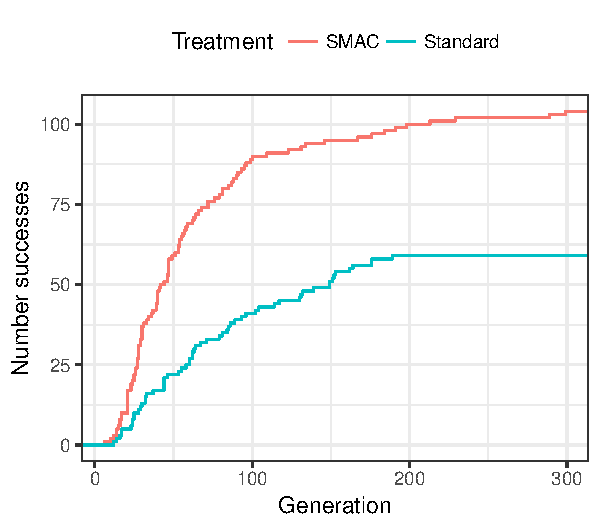
\includegraphics[width=3in]{../figures/successGenerations}
	\caption{Cumulative success counts over time for both the Standard
	and the SMAC parameter settings.}
	\label{fig:successGenerations}
\end{figure}

As Figure~\ref{fig:successGenerations} illustrates, the runs using the SMAC
parameter configuration also discovered solutions much earlier than runs using
the Standard parameters. By generation 100, for example, 90 of the 110 SMAC 
runs (or 87\%) had succeeded, where only 41 of the 110 Standard runs 
(or 37\%) had succeeded. All the pairwise (by generation) differences 
between SMAC and Standard cumulative counts in 
Figure~\ref{fig:successGenerations} are 
statistically significant ($p<0.015$)
from generation 29 forward.\footnote{Using a $\chi^2$ test of proportions 
	with the Holm correction for the 300 separate comparisons.}

\subsection{Impact of SMAC settings on genetic operator proportions}
\label{sec:SMACimpactRSWNops}

Key differences between the Standard parameter settings to the SMAC parameters
are the changes in the genetic operator probabilities, as outlined in
Table~\ref{tab:clojushParameters}. 
A question this raises is how these changes
actually impact the dynamics of the resulting runs, and in particular if and
how they affect the likelihood of a given genetic operator playing a key
role in the ultimate discovery of a solution.

%\todo{We should replace this graph with one with a more sensible shaping (e.g., width proportional to the number of genes passed to the child). We may also
%	want to have two graphs, one filtered and one not filtered to illustrate those
%	two approaches. It would also be nice if the edges were thicker/more prominent.}

\begin{figure*}
	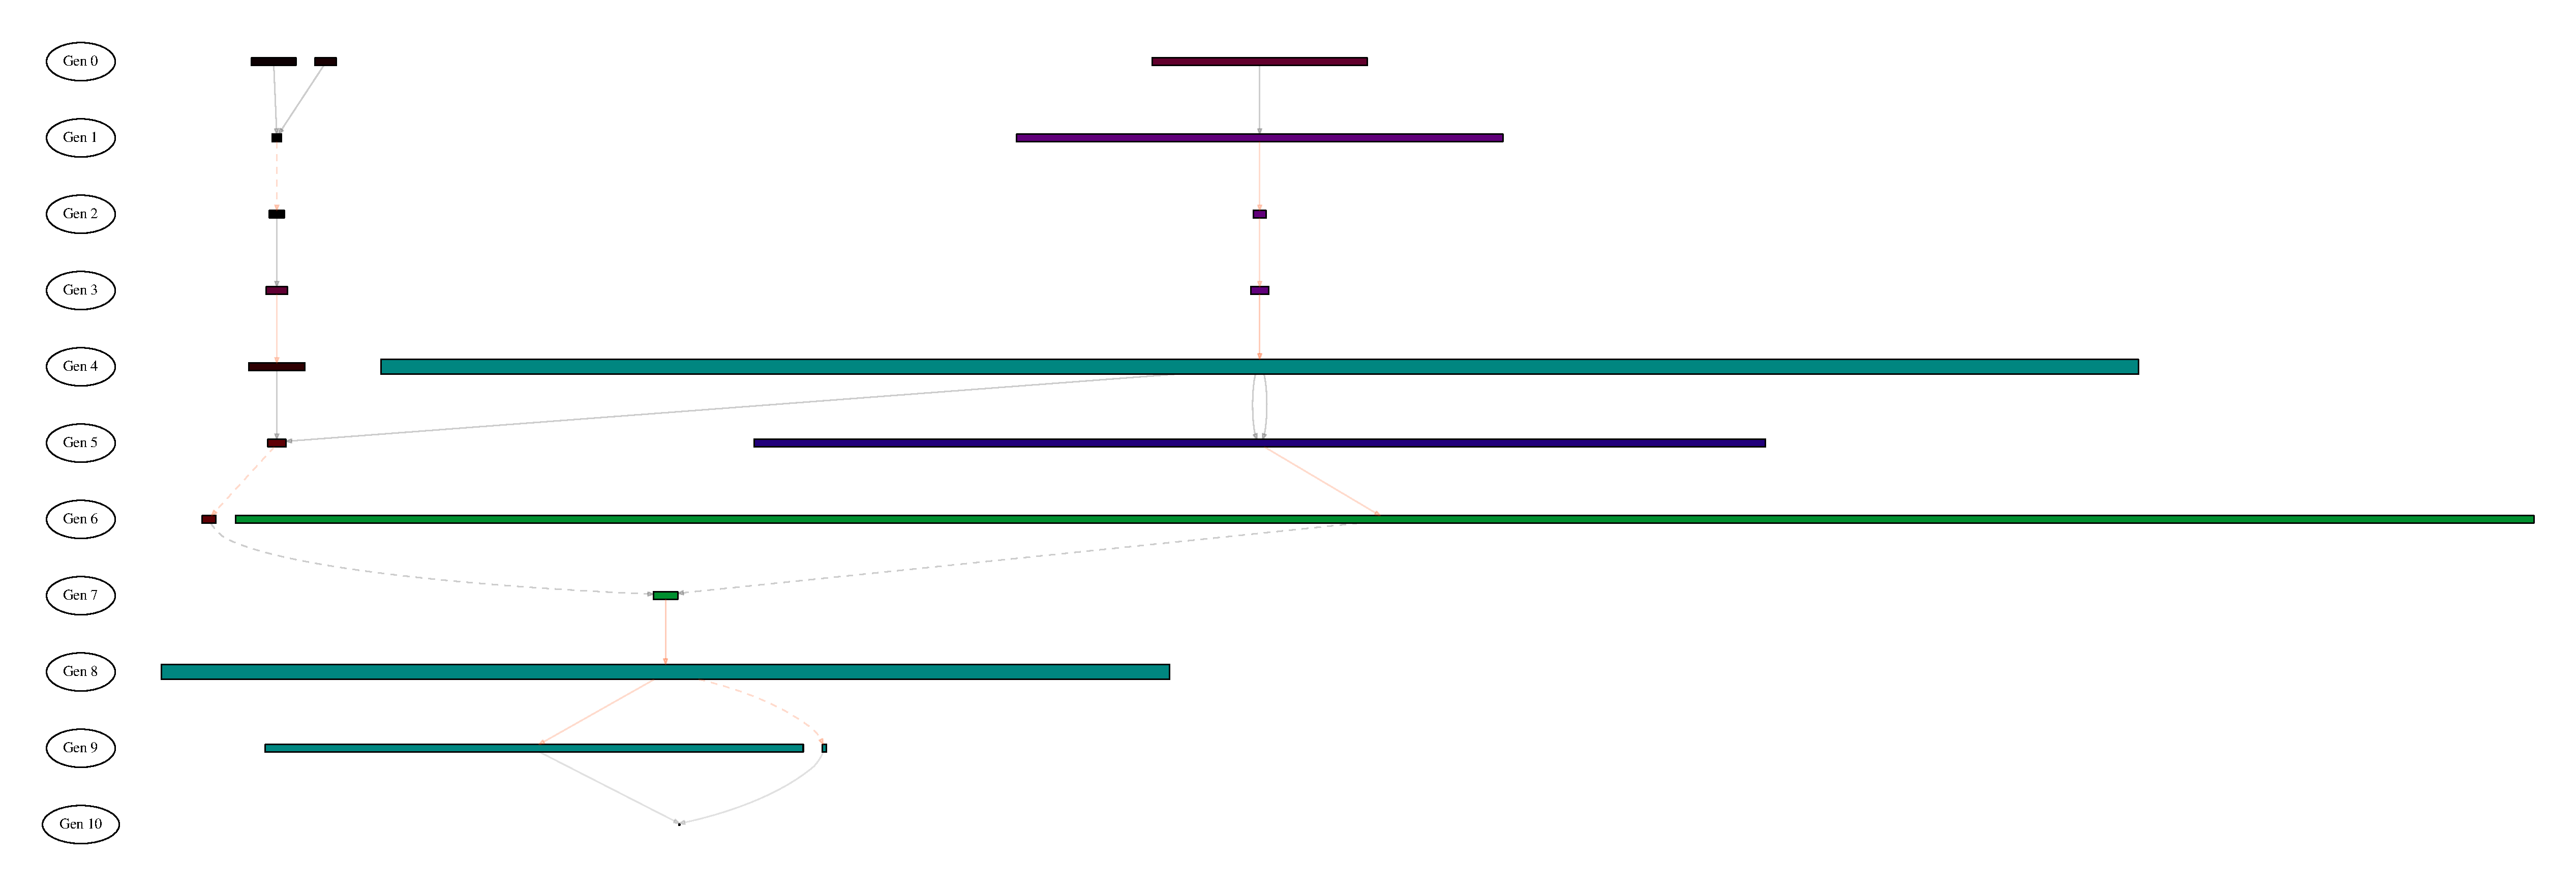
\includegraphics[width=\textwidth]{../figures/log1_filter_by_genes_vanilla}
	\caption{Ancestry graph of a successful Replace Space By Newline run
	using the ``tuned'' parameters discovered by SMAC. This tree is filtered 
	to only include individuals that ultimately passed a gene
	on to the winning individual. Each individual is represented as a
	rectangle whose width is proportional to the number of selections
	it received, and whose color is a function of its error vector.
	Edges indicate parent-child relationships. Dashed black edges indicate
	that the child was constructed via alternation alone; solid black edges 
	indicate alternation followed by uniform mutation. Solid orange edges
	indicate applications of uniform mutation, and dashed orange represent
	applications of uniform close mutation.}
	\label{fig:log1ByGenes}
\end{figure*}

To address this question, we did 10 runs of Replace Space With Newline (RSWN) 
using the Standard parameters and 10 using the SMAC parameters, 
collecting highly detailed records of parent-child relationships 
among individuals, as well as information on which genes in the Plush 
genomes of parents were copied into
the genomes of their children. This allowed us to compute full ancestry
graphs for 
runs~\cite{McPhee:2016:VGP:2908961.2931741,McPhee:2015:GPTP,McPhee:2016:GPTP},
tracing back from the ``winning'' individuals (programs that have zero error)
to discover all their ancestors. Figure~\ref{fig:log1ByGenes}, for example,
shows the (filtered) ancestry graph for one successful RSWN run 
using the SMAC parameters. Of these 20 runs with detailed data collection,
9 of the 10 runs using the SMAC parameters were successful, and 5 of the
10 runs using the Standard parameters were successful.

We know that across all the thousands of generated individuals in a run,
the proportions of the various genetic operators should at least roughly
match those in Table~\ref{tab:clojushParameters}. It's less clear, however,
whether the edges in the ancestry graph, i.e., the steps that ultimately led
to a successful individual, follow the same proportions. To better understand
the relationship between the parameter settings and the actual operator usage
in finding solutions, we collected parameter count data from the 14 successful
runs with detailed data collection, for each of three different 
groups of individuals:
\begin{description}
	\item[Ancestry] All individuals that were ancestors of one or more successful
	individuals in the final generation
	\item[Instruction] All individuals that contributed at least one instruction to
	one or more successful individuals in the final generation
	\item[LastGen] All 1,000 individuals in the final generation
\end{description}
The LastGen group essentially acts as a control to confirm that 
the overall operator usage matched the parameter settings. The Instruction group
addresses the fact that an individual can be an \emph{ancestor} of a
successful individual without actually contributing any genetic material
to that individual. An individual could contribute genetic material to its
child, for example, but that material could be snipped out and 
ultimately lost in subsequent
generations through repeated mutation and alternation. So the Instruction
group is the subset of the Ancestry group, where the Instruction group 
individuals have
at least one gene that is eventually transmitted to a successful individual
with its instruction intact. (Thus a gene could have its close count mutated
by a future uniform close mutation event, but the instruction component of
that gene would have to remain intact.)

\begin{figure*}
	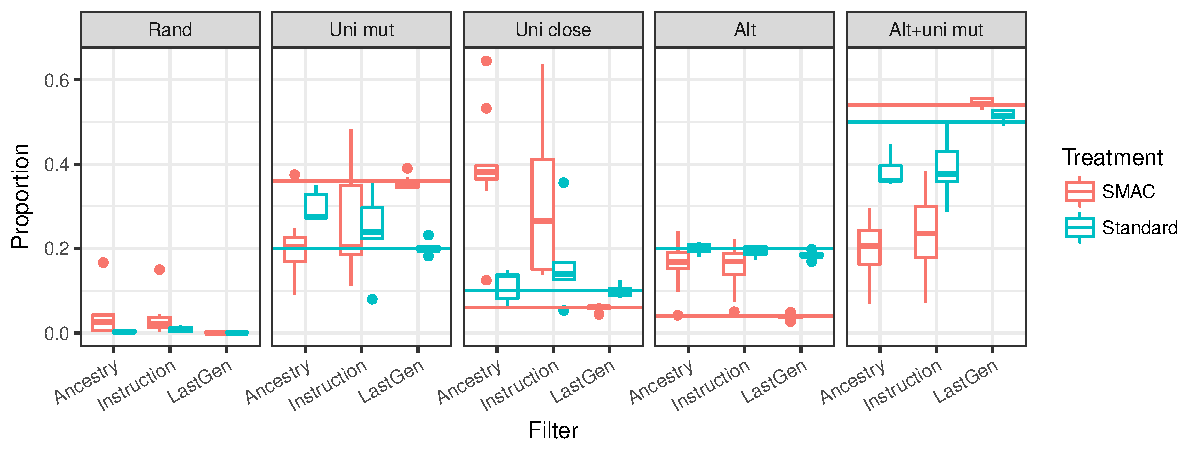
\includegraphics[width=\textwidth]{../figures/OperatorProportions}
	\caption{Proportion of the different genetic operators used to
	generate different subsets of the population. The horizontal lines 
	indicate the expected proportion of that operator as specified in 
	the parameter settings (SMAC or Standard), and deviations from those
	lines indicate places where a genetic operator was use more or less
	to generate individuals in that subset of the population 
	than we would have expected given the parameter settings. See 
	Section~\ref{sec:SMACimpactRSWNops} for additional details.}
	\label{fig:opProportions}
\end{figure*}

Figure~\ref{fig:opProportions} shows the proportion of each genetic 
operator's use in each of these three groups of the individuals, across
the 9 successful runs using the SMAC parameters, and the 5 successful runs
using the Standard parameters. The first
panel (``Random'') indicates the proportion of individuals in that collection
of individuals that were randomly generated in the initial population. 
In each of
the facets except the first (``Random''), colored horizontal lines indicate
the proportions set in the relevant parameter settings (i.e., SMAC or
Standard). Thus distributions that are substantially higher or lower than
their associated line indicate cases where the proportion of individuals in
that subset of the population created by that operation were higher or
lower than one would expect given the parameter settings.

Not surprisingly, randomly generated individuals are not a large
proportion of the individuals in either ancestry tree, and don't exist
at all in the final generation. The two SMAC outliers in the Random panel in Figure~\ref{fig:opProportions} come from the run
illustrated in Figure~\ref{fig:log1ByGenes}, which found a solution in 
just 10 generations, so the (still small) number
of ancestors in the initial random generation weren't ``amortized''
across many additional generations.

The LastGen counts are, as we would hope, close to the parameter
setting values (i.e., the horizontal lines). The fact that some of the
boxplots don't actually overlap the parameter setting is probably due
to the small number of samples, especially for Standard, where we only
have 5 successful runs.

With the exception of Standard with just Alternation and, to a
lesser degree, Standard with Uniform Close Mutation, the proportion
of operators in the either of the ancestry trees is noticeably
different from the parameter settings. For Uniform Mutation alone, for 
example, (the second panel) the SMAC parameter setting
was 0.36, but the median values across both ancestry trees were much closer to
the \emph{Standard} parameter setting of 0.2. The Standard proportions across
both ancestry trees (median 0.27 for Ancestry, 0.24 for Instruction) were definitely higher than the Standard setting of 0.2, but not as high as the
SMAC setting of 0.36. If all one had was the Standard results, one might 
have suspected that the fact that
the Standard proportions for uniform mutation were higher than the Standard
setting was a hint that successful runs would benefit from higher uniform
mutation rates. This guess would then appear to be supported by the fact
that SMAC found that a higher proportion of uniform mutation did in fact
improve success rates. What is less obvious, however, is why the \emph{actual}
proportions of uniform mutation steps that ultimate led to the discovery of
a successful individual in the SMAC runs were quite a bit lower than the SMAC
settings, being very close to the original Standard parameter value.

While it's not clear exactly what is the source of this apparent discrepancy,
one potentially contributing factor might be variations in the impact of the
different genetic operators. If, for example, alternation makes viable 
children more often, you would need fewer alternation events 
per reproduction event to generate a certain number of ``successful''
alternations. If, on the other hand, uniform mutation makes viable children 
less often (especially with SMAC's much higher uniform mutation rate), 
you would need more uniform mutation events to generate the
desired number of ``successful'' mutations. At this point this is just
speculation, and more data collection and analysis would be needed to better
understand these interactions.

\section{Applying those parameters to other problems}
\label{sec:applyingToOtherProblems}

%These are the parameters I'm using, which are approximately those taken from Nic's SMAC optimizations on RSWN:
%
%\begin{verbatim}
%:uniform-mutation-rate 0.18
%:alignment-deviation 120
%:genetic-operator-probabilities {:alternation 0.04
%                                 :uniform-mutation 0.36
%                                 :uniform-close-mutation 0.06
%                                 [:alternation :uniform-mutation] 0.54}
%\end{verbatim}
%
%All other pushgp parameters are set to default, including population size of 1000.

\begin{table}[t]
\centering
\caption{Number of successful programs out of 100 runs with standard parameters (those in the ``Default'' column of Table~\ref{tab:clojushParameters}), and with the parameters that SMAC found when run on RSWN.}
\label{table:results}
%\rowcolors{3}{Gray}{white}
\begin{tabular}{l r r}
\toprule
\textbf{Problem} & \textbf{Standard} & \textbf{SMAC} \tabularnewline
\midrule
\textit{Replace Space with Newline} & \textit{54} & \textit{91} \tabularnewline
Double Letters	& 0 & 6 \tabularnewline
String Lengths Backwards & 68 & 75 \tabularnewline
Syllables & 22 & 17 \tabularnewline
X-Word Lines & 17 & 3 \tabularnewline
\bottomrule
\end{tabular}
\end{table}

One of the hopes of using SMAC is that parameters found when optimizing one problem might be transferable to other problems with similar requirements. To test whether the parameters we found with SMAC on RSWN can be helpful for other problems, we conducted sets of 100 runs on 4 other problems from the same program synthesis benchmark suite: Double Letters, Stirng Lengths Backwards, Syllables, and X-Word Lines. Each of these problems requires a solution program that manipulates strings like RSWN, but otherwise has different requirements. For example, the Syllables problem requires the program to count the number of vowels in a given input string.

In Table~\ref{table:results} we present the number of successful runs out of 100 for each problem, using both the default parameters and those found with SMAC on RSWN. Note that we only count a program as a success if it generalizes to an unseen set of test data. Of these results, the SMAC parameters are only significantly better on the Double Letters problem.\footnote{Using a $\chi^2$ test of proportions with a significance level of $0.05$.} 
Conversely, SMAC's settings gave significantly worse resutls on the X-Word Lines problem, and no significant difference on the other two problems.

These results indicate that while the parameters discovered by SMAC on RSWN do significantly improve results on RSWN itself, they do not provide any improvements on other similar problems. This leads to the conclusion that there is some characteristic of the RSWN problem that makes high mutation rates and high alignment deviations able to find solutions much more quickly, and that this characteristic does not hold for other similar types of problems


\section{Discussion}
\label{sec:discussion}

Talk about what we learned and what this means

A piece from @thelmuth at Discourse that we might want to use:
\begin{quote}
	Here's a simpler version of my first explanation: alternation makes viable children more often, so you need less of it per event that you want to be successful. Uniform mutation makes viable children less often, so you need more of it per event that you want to be successful. Uniform close mutation makes viable children the most often, so you need least of it per event you want to be successful. Then, in the ancestors of the solution, you get the percents of the events you want to be successful, not the percent of the events you have in total.
\end{quote}

\section{Future work}
\label{sec:futureWork}

\begin{itemize}
	\item Use SMAC to tune parameters on the other four problems one at a time, and see how that works on the other problems.
	\item Use SMAC to tune on (sub)sets of the problems, like all 5, or on subsets that seem similar (or different) based on the individual tuning.
	\item etc.
\end{itemize}

\section{Conclusions}
\label{sec:conclusion}

It is important to keep in mind that there is little in this paper that is
specific to SMAC or its details or, for that matter, Clojush or its details. 
There are many approaches to parameter
tuning, and presumably similar results could have been acquired with many of
them. What matters the most here is that:
\begin{itemize}
	\item SMAC was able to discover parameter settings that 
	\emph{substantially} improved the performance
	of Clojush on the Replace Space With Newline problem.
	\item Applying those optimized parameter settings to a variety of other
	problems let to very mixed results, suggesting that those parameter
	settings were very specific to the particular problem used for the SMAC
	search.
\end{itemize}
The fact that SMAC was able to discover settings that improved
performance on the Replace Space With Newline problem by such a wide margin
is quite impressive. The fact that those parameter settings don't appear to
generalize is in no way the ``fault'' of SMAC, and are likely more 
about the computational properties of our test problems and how we used 
the tool than any property of the tool itself.

\todo[inline]{Say something about computational cost of doing suites of
problems.}
